% Template for Cogsci submission with R Markdown

% Stuff changed from original Markdown PLOS Template
\documentclass[10pt, letterpaper]{article}

\usepackage{cogsci}
\usepackage{pslatex}
\usepackage{float}
\usepackage{caption}

% amsmath package, useful for mathematical formulas
\usepackage{amsmath}

% amssymb package, useful for mathematical symbols
\usepackage{amssymb}

% hyperref package, useful for hyperlinks
\usepackage{hyperref}

% graphicx package, useful for including eps and pdf graphics
% include graphics with the command \includegraphics
\usepackage{graphicx}

% Sweave(-like)
\usepackage{fancyvrb}
\DefineVerbatimEnvironment{Sinput}{Verbatim}{fontshape=sl}
\DefineVerbatimEnvironment{Soutput}{Verbatim}{}
\DefineVerbatimEnvironment{Scode}{Verbatim}{fontshape=sl}
\newenvironment{Schunk}{}{}
\DefineVerbatimEnvironment{Code}{Verbatim}{}
\DefineVerbatimEnvironment{CodeInput}{Verbatim}{fontshape=sl}
\DefineVerbatimEnvironment{CodeOutput}{Verbatim}{}
\newenvironment{CodeChunk}{}{}

% cite package, to clean up citations in the main text. Do not remove.
\usepackage{cite}

\usepackage{color}

% Use doublespacing - comment out for single spacing
%\usepackage{setspace}
%\doublespacing


% % Text layout
% \topmargin 0.0cm
% \oddsidemargin 0.5cm
% \evensidemargin 0.5cm
% \textwidth 16cm
% \textheight 21cm

\title{Balancing informational and social goals in active learning}


\author{{\large \bf Erica J. Yoon*}, {\large \bf Kyle MacDonald*}, {\large \bf Mika Asaba}, {\large \bf Hyowon Gweon}, \and {\large \bf Michael C. Frank} \\ \{ejyoon, kylem4, masaba, hyo, mcfrank\} @stanford.edu \\ Department of Psychology, Stanford University \\ *These authors contributed equally to this work.}

\begin{document}

\maketitle

\begin{abstract}
Our actions shape what we learn. Recent work suggests that people engage
in efficient self-directed learning to maximize information gain.
However, human learning often unfolds in social contexts where learners
not only face informational goals (e.g., learn how something works) but
also social goals (e.g., appear competent and impress others). How do
these factors shape learners' decisions? Here, we present a
computational model that integrates the value of social and information
goals to predict the decisions that people will make in a simple active
causal learning task. We show that an emphasis on performance or
self-presentation goals leads to reduced chances of learning (E1) and
that social context can push learners to pursue performance-oriented
actions even when the learning goal is highlighted (E2). Our formal
model of social-active learning successfully captures the empirical
results. These findings are the first steps towards understanding the
role of social reasoning in active learning contexts.

\textbf{Keywords:}
active learning; social reasoning; information gain; OED;
self-presentation; goal tradeoffs
\end{abstract}

\section{Introduction}\label{introduction}

Imagine you are a novice cook and you have to decide what meal to
prepare for a first date. Should you choose an easy favorite or should
you attempt to make something new? While the familiar recipe can ensure
a good meal, you may miss out on a new, delicious dish. The new recipe
might taste even better, but it has a higher chance of failure. In such
\emph{explore-exploit} dilemma (Sutton \& Barto, 1998), you can choose
between \emph{exploring} the new recipe that may or may not result in a
more delicious dish (\emph{learning} goal), or \emph{exploiting} your
previous experience and knowledge to ensure a good meal
(\emph{performance} goal). Here, we explore the idea of formalizing the
learning-performance goal tradeoff using a simple active learning
context, where social factors may shape the goals we consider.

Active learning occurs when people have control over the sequence of
information in a learning context (e.g., try pressing buttons on a toy,
one by one, to see their effect). The key assumption is learners will
maximize the usefulness of their actions by gathering information that
is especially helpful for their own learning. Active contexts lead to
faster learning than passive contexts where people don't have control
over the information flow, as suggested by empirical work in education
(Grabinger \& Dunlap, 1995), machine learning (Settles, 2012), and
cognitive psychology (Castro et al., 2009).

But real-world learning usually takes place in rich social contexts with
teachers, peers, or other people who can directly influence our
learning. Indeed, children and adults seem to modulate their inferences
depending on whether evidence is generated on their own or by others
(e.g., Xu \& Tenenbaum, 2007); whether they observe intentional versus
accidental actions (Carpenter, Akhtar, \& Tomasello, 1998); and whether
they believe another person selected their actions with the goal of
helping them learn (i.e., teaching; Shafto, Goodman, \& Frank, 2012).
But even when we learn from \emph{our} own actions instead of others',
our social environment may affect our self-directed learning process.
While previous models have captured how we optimize learning, either
from our own actions or from others, they have been agnostic to other
social factors that are ubiquitous in a learner's environment. People
must integrate the value of social goals (e.g., looking competent or
knowledgeable) and information goals when deciding what to do next.

How can active learning models accommodate this richer set of utilities?
As a step towards answering this question, we model a learner who
considers a mixture of learning and performance goals. A key assumption
underlying recent Bayesian models of human social cognition is that
people expect others to act approximately optimally given a utility
function (e.g., Goodman \& Frank, 2016; Jara-Ettinger, Gweon, Schulz, \&
Tenenbaum, 2016). Our model adopts the same utility-theoretic approach,
and assumes an agent who reasons about the utility function that
represents a weighted combination of multiple goals (Yoon, Tessler,
Goodman, \& Frank, 2017) in a social active learning context.

\begin{CodeChunk}
\begin{figure}[b]

{\centering 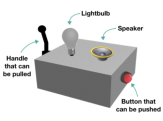
\includegraphics[width=0.65\linewidth]{figs/toy-1} 

}

\caption[An example of the toy used in our paradigm]{An example of the toy used in our paradigm.}\label{fig:toy}
\end{figure}
\end{CodeChunk}

\begin{CodeChunk}
\begin{figure*}[tb]

{\centering 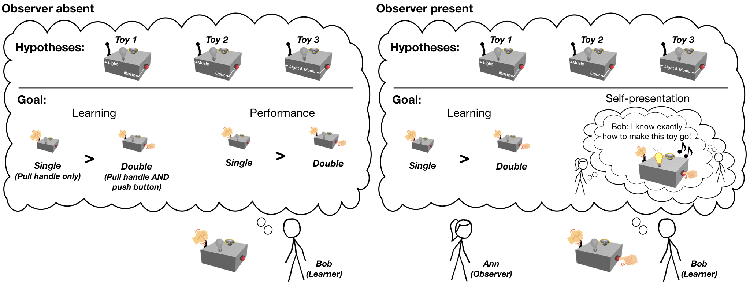
\includegraphics[width=0.95\linewidth]{figs/model_diagram-1} 

}

\caption[Diagram of the computational model]{Diagram of the computational model. The learner considers possible hypotheses: Toy 1 (handle pull turns on the light, button press turns on music, both actions cause both effects); Toy 2 (handle pull turns on music, button press turns on the light, both actions cause both effects); and Toy 3 (both actions cause both effects, but each action on its own does not produce any effect). The learner also considers his goals. When an observer is absent, he considers his learning goal and performance goal and chooses an action. The learning goal favors a single action (e.g., pull the handle only) that can fully disambiguate, whereas the performance goal favors the both action (pull the handle AND push the button) that guarantees the most salient reward. When an observer is present, the learner considers the learning, performance (not shown), and presentational goal.}\label{fig:model_diagram}
\end{figure*}
\end{CodeChunk}

We instantiate our model in a simple causal learning task and examine
how people choose actions that support learning vs.~performance goals in
different social contexts. We present a toy with an uncertain causal
mechanism (Fig \ref{fig:toy}). For this toy, doing only one of the two
possible actions (handle pull or button press) disambiguates its causal
mechanism but potentially risks no immediate effect (i.e., neither sound
nor light turning on), while doing both actions at the same time is
immediately rewarding but is not informative for learning the toy's
causal mechanism. Thus, the learner can choose between the two actions
that will each lead to one outcome (new discovery; learning) or the
other (immediate reward; performance). The learner's action rests on
relative utilities he assigns to exploration versus exploitation, which
in turn are determined in part by the social context (e.g., the presence
or absence of his
boss).\footnote{From here on, we use a male pronoun for Bob, the learner, and female pronoun for Ann, the boss and observer.}

In two experiments, we show that emphasizing performance or
self-presentation (social) goals leads to actions that are not
informative and thus reduce the chances of learning (E1). Next, we show
that the presence of an observer (i.e., a boss) pushes learners to
pursue performance/presentation-oriented actions even when the learning
goal is highlighted (E2). Finally, we show that the empirical results
are consistent with predictions of our cognitive model of social-active
learning.

\section{Computational model}\label{computational-model}

We model a learner \(L\) who chooses his action \(a\) approximately
optimally (as per optimality \(\lambda\)) based on the expected total
utility \(U_{t}\) given his action and observer presence.
\[ P_L(a | o) \propto \exp(\lambda \cdot \mathbb{E}[U_{total}(a,o)])\]
\[U_{t}(a,o) = \phi_{learn} \cdot U_{learn}(a) + \phi_{perf} \cdot U_{perf}(a) + \delta^o \cdot \phi_{pres} \cdot U_{pres}(a)\]
\noindent
where \(\phi\)s are weights that are inferred for each utility from data
and \(\delta^o\) a dirac function that is 1 if there is an observer, and
0 if there is no observer. Below we describe each utility structure (see
Fig \ref{fig:model_diagram} for a visual schematic of the model).

\subsubsection{Learning utility}\label{learning-utility}

The \emph{learning utility} symbolizes the goal to learn new
information, which in our paradigm is associated with figuring out how a
given toy works. The learning utility is formally represented by an OED
model (Lindley, 1956; ``Optimal Experiment Design''; Nelson, 2005),
which quantifies the expected utility of different information seeking
actions. The learner considers the hypothesis space \(H\), and wants to
determine the correct hypothesis. He thinks about the utility of the
outcome \(m\) to each possible action, which is equal to the
\emph{information gain}: the change in the learner's overall uncertainty
(difference in entropy) before and after seeing the outcome. This
information gain is equal to the learning utility (\(U_{learn}\)), which
is the expected utility of each action:
\[ U_{learn}(a) = \sum_{\{m, \neg m\}}{P(m|a)}[{ent(H) - ent(H|m,a)}]\]
\noindent
where \(ent(H)\) is the Shannon entropy of \(H\), which provides a
measure of the overall amount of uncertainty in the learner's beliefs
about the candidate hypothesis (MacKay, 2003). Once the learner chooses
an action \(a\), which yields an effect \(m\) (or no effect \(\neg m\)),
then he updates his beliefs about each hypothesis via standard Bayesian
updating. Finally, we scale the utility by \(log_2n\), where \(n\) is
the number of possible actions, to convert the entropy to a value
between 0 and 1.

\subsubsection{Performance utility}\label{performance-utility}

The \emph{performance utility} is the utility of achieving an immediate
rewarding outcome. Within our paradigm, the learner gains utility from
an immediate effect of music or light turning on. The expected
performance utility (\(U_{perf}\)) before the learner chooses an action
is the likelihood of an effect \(m\) given the action \(a\).
\[ U_{perf} = P_L(m | a) \] \noindent

\subsubsection{Presentation utility}\label{presentation-utility}

When there is another person present to observe the learner's action,
the observer \(O\) is expected to reason about the learner \(L\)'s
competence, equal to whether the learner was able to make the toy
produce an effect. The learner thinks about the observer's inferential
process, and the expected \emph{presentational} utility (\(U_{pres}\))
is based on maximizing the apparent competence inferred by the observer.
\[ U_{pres} = P_O(m | a)\] \noindent
where \(P_O(m | a)\) is the observer's own estimate of the likelihood of
an effect given the learner's action.

\section{Experiment 1}\label{experiment-1}

In Experiment 1 (E1), we first wanted to confirm that participants would
choose different actions depending on what goal was highlighted. We were
also interested in how people would act when no explicit goal was
specified within the task. Participants were asked to act on a toy with
an uncertain causal mechanism, and were assigned to different goal
conditions: (1) learning (learn how the toy works), (2) performance
(make the toy play music), (3) presentation (impress their boss), and
(4) no goal specified. We hypothesized that participants would choose an
informative action more often in the following order of goal conditions
(decreasing): learning, no goal, performance, and
presentation.\footnote{Our hypothesis, method, model and data analysis were pre-registered prior to data collection at \url{https://osf.io/kcjau}.}

\begin{CodeChunk}
\begin{figure*}[tb]

{\centering 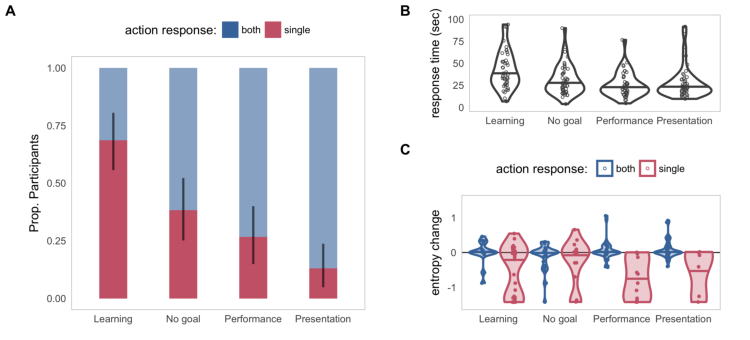
\includegraphics[width=0.95\linewidth]{figs/e1_behav_results_plot-1} 

}

\caption[Behavioral results for E1]{Behavioral results for E1. A: Proportion of action decisions for each goal condition. Error bars represent 95\% binomial CIs computed using a Bayesian beta-binomial model. B: Participants' response times on the action decisions. Each point represents a participant with the width of the violin representing the density of the data at that value. C: Participants' belief change (entropy in bits) as a function of condition. Lower values represent higher certainty after selecting an action.}\label{fig:e1_behav_results_plot}
\end{figure*}
\end{CodeChunk}

\subsection{Method}\label{method}

\subsubsection{Participants}\label{participants}

We recruited 196 participants (45-51 per condition) on Amazon's
Mechanical Turk, with IP addresses in the US and a task approval rate
above 85\%. We excluded 7 participants who failed to answer at least two
out of three manipulation check questions correctly (see Procedure
section for details on the manipulation check), and thus the remaining
189 participants were included in our final analysis.

\subsubsection{Stimuli and Design}\label{stimuli-and-design}

We presented images and instructions for three different toys that
looked very similar but worked in different ways (see captions for Fig
\ref{fig:model_diagram}). The instructions conveyed that pressing the
button and pulling the handle was immediately rewarding but
uninformative (fails to disambiguate the causal mechanism). In contrast,
either of the single actions was completely disambiguating, but was
uncertain to produce an immediate outcome. Each toy had a label at the
front, indicating the correct action(s)--outcome link.

We asked participants to act on one of these toys; importantly, the
given toy was missing its label, leading to uncertainty about its causal
structure. We randomly assigned participants into four goal conditions.
In the \emph{No-Goal} condition we did not specify any goal for
participants. In the \emph{Learning}, \emph{Performance}, and
\emph{Presentation} conditions, we asked participants to imagine they
were toy developers and one day their boss approached them. We
instructed participants to: figure out the correct label for the toy
(\emph{Learning}); make the toy play music (or turn the light on;
\emph{Performance}); or impress their boss and show that they are
competent (\emph{Presentation}). We asked participants to select an
action out of the following set: ``press the button'', ``pull the
handle'', or ``press the button and pull the handle.'' The order of
actions was randomized.

\subsubsection{Procedure}\label{procedure}

In the \emph{exposure phase}, we showed participants an example toy and
gave instructions for three toy types. We first presented the
instructions for the single action toys (Toy 1 and Toy 2) in a
randomized order, and then presented the instructions for the both
action toy (Toy 3). After instructions, participants indicated what
action would make each toy operate (e.g., ``How would you make
{[}this{]} toy play music?'') to show that they understood how the
different toys worked.

In the \emph{test phase}, participants read a scenario for one of the
four goal conditions, followed by the question: ``If you only had one
chance to try a SINGLE action {[}to pursue the specified goal{]}, which
action would you want to take? You will get a 10 cent bonus \ldots{} if
you {[}achieve the given goal{]}''.

Both before and after the critical action decision trial, we asked
participants to rate the likelihood that the unknown toy was Toy 1, 2,
or 3, which indexed participants' prior beliefs about how the toys were
likely to function and their \emph{belief change} after selecting an
action and observing its effect.

\subsection{Results and discussion}\label{results-and-discussion}

\subsubsection{Action decisions:}\label{action-decisions}

We modeled action decisions using a logistic regression
\texttt{$action \sim goal\_condition$} with the No-goal condition as the
reference
category.\footnote{In all of the analyses for E1 and E2, we used the {\fontfamily{qcr}\selectfont rstanarm} package to fit Bayesian regression models estimating the differences across conditions. We report the uncertainty in our point estimates using 95\% Highest Density Intervals (HDI). The HDI provides a range of credible values given the data and model.}
Participants' tendency to select a ``single'' action varied across
conditions as predicted (Fig \ref{fig:e1_behav_results_plot}A), with the
highest proportion in the Learning condition, followed by No-goal,
Performance, and Presentation.

Compared to the No-goal condition, participants selected the single
action at a greater rate in the Learning condition (\(\beta\) = 1.28,
{[}0.5, 2.17{]}) and at lower rate in the Presentation context
(\(\beta\) = -1.41, {[}-2.47, -0.4{]}), with the null value of zero
difference condition falling well outside the 95\% HDI, and at similar
rate in the Performance condition (\(\beta\) = -0.53, {[}-1.43, 0.35{]})
with the 95\% HDI including the null.

\subsubsection{Action decision times:}\label{action-decision-times}

We analyzed decision times, which were the latency to make an action
selection as measured from the start of the action decision trial (all
RTs were analyzed in log space), using the same model specification as
action decisions. Fig \ref{fig:e1_behav_results_plot}A shows the full RT
data distribution. Compared to the No-Goal condition (\(M\)= 31
seconds), participants took on on average 12.2 (4.2, 20) seconds longer
to generate a decision in the Learning condition. In contrast,
participants in the Performance and Presentation conditions produced
similar decision times.

\subsubsection{Belief change:}\label{belief-change}

We quantified participants' beliefs about the toy using entropy, and
belief change was measured as the difference in entropy before and after
selecting an action. We modeled change in entropy as a function of goal
condition and participants' action choices:
\texttt{$entropy\_change \sim goal\_condition + action\_response$} (Fig
\ref{fig:e1_behav_results_plot}C). Across all conditions, people who
selected the single action showed a greater reduction in entropy
(\(\beta\) = -0.49, {[}-0.64, -0.33{]}, i.e., learned more from their
action. We did not see evidence of an interaction between goal and
action selection. However, a larger proportion of participants selected
a single action in the Learning context, so learning was more likely in
this scenario.

\begin{CodeChunk}
\begin{figure*}[tb]

{\centering 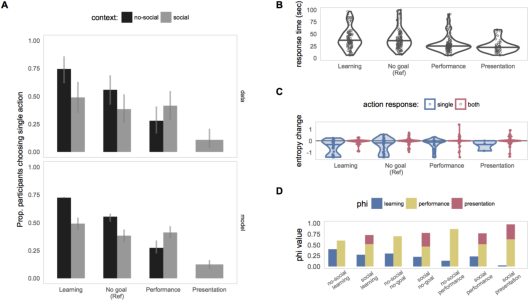
\includegraphics[width=0.95\linewidth]{figs/e2_results-1} 

}

\caption[Behavioral and model fitting results for E2]{Behavioral and model fitting results for E2. A: Action decisions with color representing social context, from human data (top) and fitted model predictions (bottom). B: Decision times. C: Belief change. D: Inferred phi values for each goal-context condition. All other plotting conventions are the same as Fig 3.}\label{fig:e2_results}
\end{figure*}
\end{CodeChunk}

\section{Experiment 2}\label{experiment-2}

In E1, we confirmed that participants selected different actions
depending on the type of goal emphasized. In E2, our goals were
three-fold: (1) to replicate the results from E1; (2) to manipulate
goals \emph{and} the presence/absence of another person
(social/no-social) independently, allowing us to measure the interaction
between goals and social context; and (3) to compare empirical data with
predictions of our computational model. Our key behavioral prediction
was an interaction: that participants would be less likely to select a
single (more informative) action in the Learning goal and No-goal
conditions when their boss was present. We also predicted a null result:
that the presence of the boss should not affect action decisions in the
Performance condition.

\subsection{Method}\label{method-1}

\subsubsection{Participants}\label{participants-1}

Using the same recruitment and exclusion criteria as E1, we recruited
347 participants (42-51 per condition), and 325 participants were
included in our final analysis.

\subsubsection{Stimuli and Design}\label{stimuli-and-design-1}

The stimuli and design were identical to E1, except we had 7 different
goal \(\times\) social conditions. Goals were identical to E1; social
context varied depending on whether the boss was present (\emph{social})
or absent (\emph{no-social}) in the story. The conditions were:
\emph{Social-learning}, \emph{Social-performance},
\emph{Social-presentation}, \emph{No-social-no-goal},
\emph{No-social-learning}, \emph{No-social-performance}, and
\emph{Social-no-goal}. Note that we did not have
\emph{No-social-presentation} condition, because the presentation goal
was defined by presenting oneself as competent to another person.

\subsubsection{Procedure}\label{procedure-1}

The procedure was identical to E1.

\subsection{Results and discussion}\label{results-and-discussion-1}

\subsubsection{Action decisions:}\label{action-decisions-1}

We modeled action decisions using a logistic regression specified as
\texttt{$action \sim goal\_condition * social\_context$} with the
no-goal-no-social condition as the reference category. We replicated the
key finding from E1: participants selected a ``single'' action more
often when they were in a context that emphasized a learning goal,
followed by the no-goal, performance, and presentation conditions (Fig
\ref{fig:e2_results}A). There was a main effect of social context, with
participants being less likely to select the single action when their
boss was present (\(\beta =\) -0.521, {[}-1.005, -0.053{]}). Finally,
there was evidence for a reliable interaction between goal condition and
social context such that the effect of social context was present in the
Learning and No-Goal conditions, but not in the Performance condition
(\(\beta\) \(_{int}\) = 1.163, {[}0.01, 2.312{]}).

\subsubsection{Action decision times:}\label{action-decision-times-1}

We replicated the key decision time finding from E1, with participants
making slower decisions in the Learning context as compared to
Performance/Presentation. On average, participants took seconds to
generate a response in the No-goal condidition and seconds in the
Learning condition. In contrast, decisions were faster in the
Performance (\(\beta\) = -7.78 sec, {[}-14.01, -1.52{]}) and
Presentation (-10.77 seconds, {[}-18.67, -2.73{]}) conditions, which
were similar to one another (Fig \ref{fig:e2_results}B). There was no
evidence of a main effect of social context or an interaction between
goal condition and social context. Note that here we did not see a
difference in decision times between the Learning and No-Goal
conditions, which is different from the pattern in E1.

\subsubsection{Belief change:}\label{belief-change-1}

Across all conditions, participants who selected the single action
showed a greater reduction in entropy (\(\beta\) = -0.35, {[}-0.45,
-0.24{]}. There was weaker evidence of greater reduction in entropy in
the Learning goal condition (\(\beta\) = -0.12, {[}-0.25, 0.01). There
was no evidence of a main effect of social context and no two- or
three-way interactions between social context, goal condition, and
action choice.

\subsubsection{BDA model-data fit:}\label{bda-model-data-fit}

In our paradigm, participants chose an action based on a certain
goal.\footnote{For action priors, we used a separate prior elicitation task, in which people indicated the likelihood for selecting an action without any background information about possible hypotheses or goals. We used mean likelihood for each action choice as baseline priors in our model.}
We assumed that the goal descriptions (e.g., ``impress your boss'')
conveyed to the participants a particular set of goal weights
\{\(\phi_{learn}\), \(\phi_{perf}\), \(\phi_{pres}\)\} used to generate
action choices. We put uninformative priors on these weights
(\(\phi \sim Unif(0,1)\)) and inferred their credible values for each
social-goal condition, using Bayesian data analytic techniques (Lee \&
Wagenmakers, 2014).

The inferred goal weights were consistent with what we predicted (Fig
\ref{fig:e2_results}D). \(\phi_{learn}\) was at its highest for
No-social learning condition. On the other hand, the \(\phi_{perf}\) and
\(\phi_{pres}\) together make up the highest portion in the presentation
condition, with high social pressure to present competence compared to
other conditions.

We also inferred another parameter of the cognitive model, the
optimality parameter \(\lambda\). We put uninformative prior on the
parameter (\(\lambda \sim Unif(0,10)\) and inferred its posterior
credible value from the data. We ran 4 MCMC chains for 100,000
iterations, discarding the first 50,000 for burnin. The Maximum A-
Posteriori (MAP) estimate and 95\% Highest Probability Density Interval
(HDI) for \(\lambda\) was 4.79 {[}3.96, 6.2{]}.

The fitted model predictions of action choices are shown in Fig
\ref{fig:e2_results}A (bottom). The model's expected posteriors over
action choices capture key differences between conditions: the single
action was more likely for no-social than social conditions overall, but
not when the performance goal was highlighted. The model was able to
predict the distribution of action responses with high accuracy
\(r^2(21)\) = 0.9.

\section{General Discussion}\label{general-discussion}

How do social contexts shape active learning? We proposed that people
integrate learning-, performance-, and presentation-oriented goals when
deciding what to do. In two experiments, we showed that people chose
more informative actions, when learning goals were highlighted and in
the absence of a relevant social context (no boss present), while they
chose more immediately rewarding actions when performance or
presentational goals were highlighted, especially when a boss was
present. When no explicit goal was specified, people showed behavior
that seemed to reflect a mixture of goals. Our model of social-active
learning successfully captured key patterns in the participants' action
decisions.

This work brought active learning accounts into contact with social
learning theories. We used ideas from Optimal Experiment Design, which
models active learning as a process of rational choice that maximizes
information gain, and Bayesian modeling framework, which formalizes a
process of recursive social reasoning. Thereby we could include social
information within a formal utility-theoretic framework, building a
richer utility function that represented a weighted combination of
multiple goals -- informational and social.

There are limitations to this work that present opportunities for future
work. First, we did not differentiate between performance and
presentation goals, since the choice of doing both actions satisfies
both of these goals. Future work enriching the space of possible actions
can tease apart actions driven by self-presentation. Second, we used a
very particular social context (the presence of a boss) to influence
people's action choices. It remains an open question as to how our
results would generalize to other kinds of observers with different
goals (e.g., a teacher who wants the learner to select actions that help
her learn). Third, we limited people to a single action choice. While
this allowed a clean measurement of our condition manipulations,
real-world learning often involves sequential decision-making that could
cause learners to prioritize different goals depending on their prior
actions or the probability of interacting with an observer in the
future.

Another interesting open question is how our model could be used to
understand active learning over development. Our framework could allow
us to measure changes in children's goal preferences as they develop
better social reasoning and meta-cognitive abilities. One prediction is
that young children focus on learning goals earlier on when they are
surrounded by familiar caregivers who scaffold learning-relevant
actions. But as their social reasoning abilities mature and their social
environments become more complex, children may start to emphasize
performance or presentation goals.

Overall, this work represents a first step to answering these rich
questions that ultimately seek to unify theories on active learning and
social reasoning.

\vspace{1em}
\fbox{\parbox[b][][c]{7.3cm}{\centering All data, model, and analysis codes are available at: \url{https://github.com/kemacdonald/soc-info}}}
\vspace{1em} \noindent

\section{Acknowledgements}\label{acknowledgements}

This work was supported by an NSERC postgraduate doctoral scholarship to
EJY and an NSF GRFP to KM.

\section{References}\label{references}

\setlength{\parindent}{-0.1in} \setlength{\leftskip}{0.125in}

\noindent

\hypertarget{refs}{}
\hypertarget{ref-carpenter1998fourteen}{}
Carpenter, M., Akhtar, N., \& Tomasello, M. (1998). Fourteen-through
18-month-old infants differentially imitate intentional and accidental
actions. \emph{Infant Behavior and Development}, \emph{21}(2), 315--330.

\hypertarget{ref-castro2009human}{}
Castro, R. M., Kalish, C., Nowak, R., Qian, R., Rogers, T., \& Zhu, X.
(2009). Human active learning. In \emph{Advances in neural information
processing systems} (pp. 241--248).

\hypertarget{ref-goodman2016}{}
Goodman, N. D., \& Frank, M. C. (2016). Pragmatic language
interpretation as probabilistic inference. \emph{Trends in Cognitive
Sciences}, \emph{20}(11), 818--829.

\hypertarget{ref-grabinger1995rich}{}
Grabinger, R. S., \& Dunlap, J. C. (1995). Rich environments for active
learning: A definition. \emph{ALT-J}, \emph{3}(2), 5--34.

\hypertarget{ref-jara2016}{}
Jara-Ettinger, J., Gweon, H., Schulz, L. E., \& Tenenbaum, J. B. (2016).
The naïve utility calculus: Computational principles underlying
commonsense psychology. \emph{Trends in Cognitive Sciences},
\emph{20}(8), 589--604.

\hypertarget{ref-lee2014bayesian}{}
Lee, M. D., \& Wagenmakers, E.-J. (2014). \emph{Bayesian cognitive
modeling: A practical course}. Cambridge university press.

\hypertarget{ref-lindley1956}{}
Lindley, D. V. (1956). On a measure of the information provided by an
experiment. \emph{The Annals of Mathematical Statistics}, 986--1005.

\hypertarget{ref-mackay2003}{}
MacKay, D. J. (2003). \emph{Information theory, inference and learning
algorithms}. Cambridge university press.

\hypertarget{ref-nelson2005}{}
Nelson, J. D. (2005). Finding useful questions: On bayesian
diagnosticity, probability, impact, and information gain.
\emph{Psychological Review}, \emph{112}(4).

\hypertarget{ref-settles2012active}{}
Settles, B. (2012). Active learning. \emph{Synthesis Lectures on
Artificial Intelligence and Machine Learning}, \emph{6}(1), 1--114.

\hypertarget{ref-shafto2012learning}{}
Shafto, P., Goodman, N. D., \& Frank, M. C. (2012). Learning from
others: The consequences of psychological reasoning for human learning.
\emph{Perspectives on Psychological Science}, \emph{7}(4), 341--351.

\hypertarget{ref-sutton1998}{}
Sutton, R. S., \& Barto, A. G. (1998). \emph{Introduction to
reinforcement learning} (Vol. 135). MIT Press Cambridge.

\hypertarget{ref-xu2007}{}
Xu, F., \& Tenenbaum, J. B. (2007). Word learning as bayesian inference.
\emph{Psychological Review}, \emph{114}(2), 245.

\hypertarget{ref-yoon2017}{}
Yoon, E. J., Tessler, M. H., Goodman, N. D., \& Frank, M. C. (2017). ``I
won't lie, it wasn't amazing'': Modeling polite indirect speech. In
\emph{Proceedings of the thirty-ninth annual conference of the Cognitive
Science Society}.

\end{document}
